\begin{center}
  \Large\textbf{BIOGRAFI PENULIS}
\end{center}
\vspace{2ex}

\addcontentsline{toc}{chapter}{BIOGRAFI PENULIS}

\begin{wrapfigure}{L}{0.3\textwidth}
  \centering
  \vspace{-3ex}
  % Ubah nama file gambar berikut dengan nama file foto dari mahasiswa pertama
  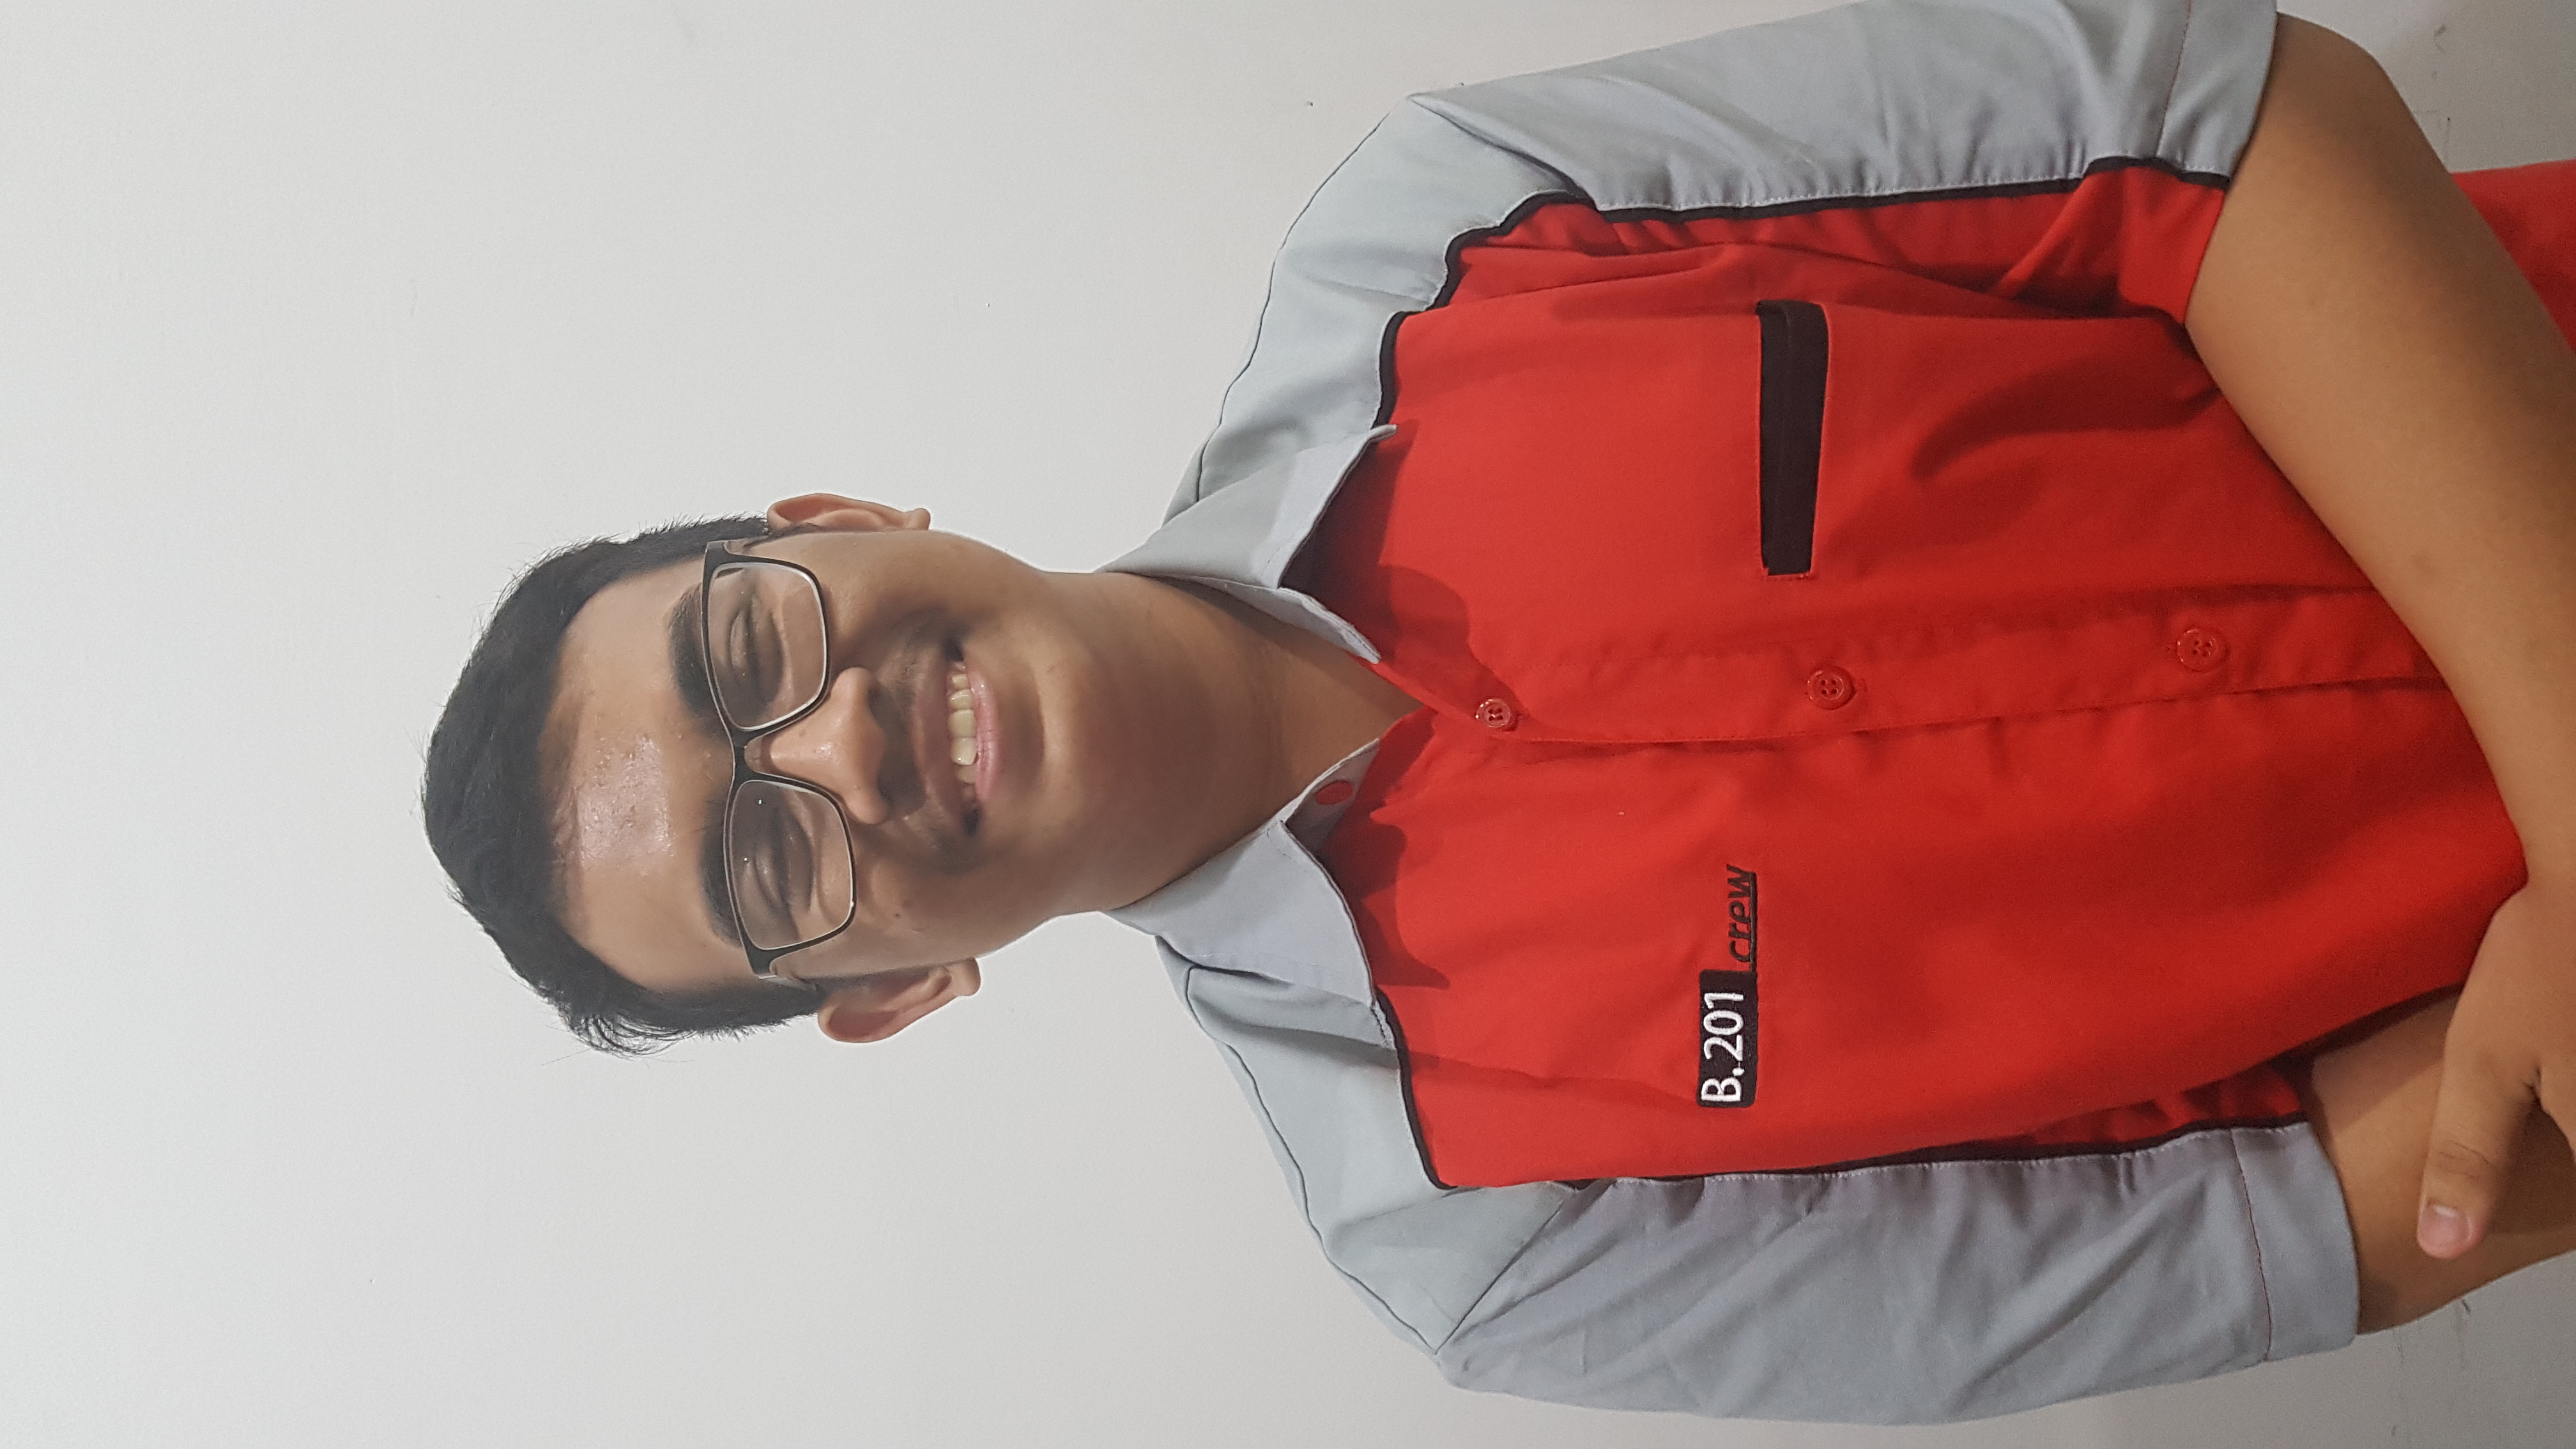
\includegraphics[width=0.5\textwidth, angle=-90]{gambar/foto.jpg}
\end{wrapfigure}

% Ubah kalimat berikut dengan biografi dari mahasiswa pertama
\noindent Aufa Nabil Amiri, lahir pada tanggal 5 Maret 2000, Surabaya. Merupakan seseorang mahasiswa yang berasal dari Institut Teknologi Sepuluh Nopember departemen Teknik Komputer. Penulis merupakan lulusan SMP Muhammadiyah 5 Surabaya dan dilanjutkan dengan SMA Negeri 2 Surabaya. Dalam masa kuliah, penulis tertarik pada bidang pengembangan \textit{Software Development}  dan Pembelajaran Mesin. Selain itu, penulis juga aktif dalam organisasi Lab B201 selama kurang 2 tahun. Penulis juga aktif dalam mengikuti kompetisi pengembangan perangkat lunak dan berhasil meraih penghargaan di ajang GEMASTIK XII 2019. Bagi pembaca yang memiliki kritik, saran, atau pertanyaan mengenai laporan magang ini dapat menghubungi penulis melalui surel aufa.nabil.amiri@gmail.com

\vspace{2ex}

% Ubah kalimat berikut dengan biografi dari mahasiswa kedua
